\documentclass[xcolor=dvipsname, handout]{beamer} %handout, ignorenonframetext

%\usepackage[ngerman]{babel}
\usepackage[utf8]{inputenc}
\usepackage{amsmath}
\usepackage{graphicx}
\usepackage{subfigure}
\usepackage{multimedia}
\usepackage{wrapfig}
\usepackage{listings}
\usepackage{comment}
\usepackage{framed,color}
\usepackage{listings}


\fboxsep=1pt%padding thickness
\fboxrule=1pt%border thickness
\usepackage{fancybox}

\usepackage{lipsum}
\usepackage{tabularx}
\usepackage{colortbl}
\usepackage{url}


\hypersetup{
	linkcolor=DarkSkyBlue,
	citecolor= DarkSkyBlue,
	filecolor= DarkSkyBlue,
	urlcolor= DarkSkyBlue
}


% COLOR-DEFINITION
%%%%%%%%%%%%%%%%%%%%%%%%
\definecolor{LightButter}{rgb}{0.98,0.91,0.31}
\definecolor{LightOrange}{rgb}{0.98,0.68,0.24}
\definecolor{LightChocolate}{rgb}{0.91,0.72,0.43}
\definecolor{LightChameleon}{rgb}{0.54,0.88,0.20}
\definecolor{LightSkyBlue}{rgb}{0.45,0.62,0.81}
\definecolor{LightPlum}{rgb}{0.68,0.50,0.66}
\definecolor{LightScarletRed}{rgb}{0.93,0.16,0.16}
\definecolor{LightGray}{rgb}{0.80,0.80,0.80}
\definecolor{Butter}{rgb}{0.93,0.86,0.25}
\definecolor{Orange}{rgb}{0.96,0.47,0.00}
\definecolor{Chocolate}{rgb}{0.75,0.49,0.07}
\definecolor{Chameleon}{rgb}{0.45,0.82,0.09}
\definecolor{SkyBlue}{rgb}{0.20,0.39,0.64}
\definecolor{Plum}{rgb}{0.46,0.31,0.48}
\definecolor{ScarletRed}{rgb}{0.80,0.00,0.00}
\definecolor{DarkButter}{rgb}{0.77,0.62,0.00}
\definecolor{DarkOrange}{rgb}{0.80,0.36,0.00}
\definecolor{DarkChocolate}{rgb}{0.56,0.35,0.01}
\definecolor{DarkChameleon}{rgb}{0.30,0.60,0.02}
\definecolor{DarkSkyBlue}{rgb}{0.12,0.29,0.53}
\definecolor{DarkPlum}{rgb}{0.36,0.21,0.40}
\definecolor{DarkScarletRed}{rgb}{0.64,0.00,0.00}



% HPI-THEME
%%%%%%%%%%%%%%%%%%%%%%%%
\RequirePackage{scrlfile}
%\ReplaceFile{beamerthemehpiswa.sty}{theme/beamerthemehpiswa.sty}
%\ReplaceFile{beamercolorthemehpiswa.sty}{theme/beamercolorthemehpiswa.sty}
%\ReplaceFile{beamerfontthemehpiswa.sty}{theme/beamerfontthemehpiswa.sty}
%\ReplaceFile{beamerinnerthemehpiswa.sty}{theme/beamerinnerthemehpiswa.sty}
%\ReplaceFile{beamerouterthemehpiswa.sty}{theme/beamerouterthemehpiswa.sty}
%\ReplaceFile{hpi.png}{theme/hpi.png}
\usetheme{hpiswa}


% BEAMER-Anpassungen
%%%%%%%%%%%%%%%%%%%%%%%%
\setbeamercolor{block title}{bg=DarkOrange}
\setbeamercolor{block body}{bg=Orange!20}
%\setbeamercolor{block title alerted}{bg=red}
\setbeamercolor{block body alerted}{bg=red!20}
%\setbeamercolor{block title example}{bg=green}
\setbeamercolor{block body example}{bg=DarkChameleon!20}
%\usecolortheme[RGB={205,173,0}]{structure}
\usecolortheme[RGB={30,74,135}]{structure}

\usecolortheme{orchid}
%\usefonttheme{professionalfonts}
%\useoutertheme[subsection=false]{smoothbars}
%\useinnertheme{rectangles}
%\setbeamertemplate{blocks}[shadow=true]

\setbeamercovered{transparent}
\setbeamertemplate{navigation symbols}{}%remove navigation symbols



% Eigene Anpassungen
%%%%%%%%%%%%%%%%%%%%

% Explainframes:
\usepackage{ifthen}
\newboolean{isexplainframe}
\setboolean{isexplainframe}{false}
\mode<handout>{
\newenvironment{explainframe}[1]{
\setboolean{isexplainframe}{true}
\addtocounter{framenumber}{-1}
\setbeamertemplate{background}[grid][step=5mm,color=LightGray]
\begin{frame}[fragile,environment=explainframe]{Handout only: #1}%
}{%
\end{frame}%
\setboolean{isexplainframe}{false}
}
\newenvironment{clearexplainframe}[0]{
\setboolean{isexplainframe}{true}
\addtocounter{framenumber}{-1}
\setbeamertemplate{background}[grid][step=5mm,color=LightGray]
\begin{frame}[fragile,environment=clearexplainframe]%
}{%
\end{frame}%
\setboolean{isexplainframe}{false}
}
}
\mode<beamer>{
\excludecomment{explainframe}
}

\setbeamertemplate{footline}{%
	\leavevmode%
	\hbox{%
		\begin{beamercolorbox}[wd=.45\paperwidth,ht=2.25ex,dp=1ex,center]{author in head/foot}%
			\usebeamerfont{author in head/foot}\insertinstitute
		\end{beamercolorbox}%
		\begin{beamercolorbox}[wd=.2\paperwidth,ht=2.25ex,dp=1ex,center]{title in head/foot}%
			\usebeamerfont{title in head/foot}\insertshorttitle
		\end{beamercolorbox}%
		\begin{beamercolorbox}[wd=.35\paperwidth,ht=2.25ex,dp=1ex,right]{date in head/foot}%
			\usebeamerfont{date in head/foot}\insertshortdate{}\hspace*{2em}
			\insertframenumber{}\ifthenelse{\boolean{isexplainframe}}{E}{} / \inserttotalframenumber\hspace*{2ex}
	\end{beamercolorbox}}%
	\vskip0pt%
}

\definecolor{javared}{rgb}{0.6,0,0} % for strings
\definecolor{javagreen}{rgb}{0.25,0.5,0.35} % comments
\definecolor{javapurple}{rgb}{0.5,0,0.35} % keywords
\definecolor{javadocblue}{rgb}{0.25,0.35,0.75} % javadoc

\lstset{
  language=Ruby,
  basicstyle=\scriptsize\ttfamily,
  keywordstyle=\color{javapurple}\bfseries,
  stringstyle=\color{javared},
  commentstyle=\color{javagreen},
  morecomment=[s][\color{javadocblue}]{/**}{*/},
  tabsize=4,
  showspaces=false,
  showstringspaces=false,
  breaklines=true
}


% Gliederung vor jedem Punkt:
\AtBeginSection[]{
\ifthenelse{\equal{\value{section}}{1}}{}{
\ifthenelse{\equal{\value{section}}{6}}{}{
\begin{frame}{Overview}
	\tableofcontents[currentsection, hideothersubsections]
\end{frame}
}
}
}


% Quote-Environment:

\renewenvironment{quote}{%
\begin{exampleblock}{}%
\begin{center}%
\begin{large}%
``}{%
''\end{large}%
\end{center}%
\end{exampleblock}}




% Dokument-Meta-Daten:
%%%%%%%%%%%%%%%%%%%%%%%
\title{Nested Class for Squeak/Smalltalk}
\subtitle{Seminar Module Systems, SS2015}
\author{Jan Graichen, Bastian Kruck, Fabio Niephaus, Matthias Springer}
\date{\today}
\institute[2015]{Software Architecture Group, Hasso Plattner Institute}



\begin{document}

\begin{frame}[plain]
	\maketitle
\end{frame}
\begin{frame}{Overview}
	\tableofcontents[hideallsubsections]
\end{frame}


\section{Introduction}

\begin{frame}{Modularity}
\begin{table}
TODO: add definition of modularity
\end{table}
\end{frame}

\begin{frame}{Recap: Newspeak Nested Classes}
  \begin{itemize}
    \item Class = methods + nested classes + slots (instance variables).
    \item Late Binding: all references to class names are self sends.
    \item External Configuration: \texttt{platform} object contains external dependencies.
    \item Lookup: lexical scope, then inheritance chain.
  \end{itemize}
\end{frame}

\section{Concept}
\begin{frame}{Goals}
  \begin{itemize}
    \item Better \textbf{understandability} and \textbf{readability} through hierarchical decomposition.
    \item More and fine-grained \textbf{code reuse} through mixin modularity (modules).
    \item \textbf{Resource management} with resources as class members.
    \item Avoiding \textbf{class name clashes} with classes as namespaces.
    \item Later (?): avoiding \textbf{extension method clashes} with COP layers.
  \end{itemize}
\end{frame}

\begin{frame}[fragile]{Nested Classes in Squeak}
\begin{minipage}{.5\textwidth}
  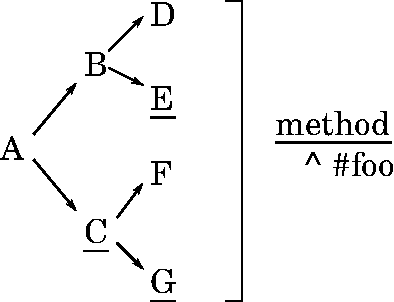
\includegraphics[width=\textwidth]{nested_classes.pdf}
\end{minipage}% This must go next to `\end{minipage}`
\begin{minipage}{.1\textwidth}
\qquad
\end{minipage}% This must go next to `\end{minipage}`
\begin{minipage}{.4\textwidth}
  \begin{lstlisting}
A new B new D method.

A new B E method.

A C new F method.

A C G method.


  \end{lstlisting}
(UML notation)

\end{minipage}


\end{frame}

\section{Use Cases}
\begin{frame}{Use Cases}
  \centering
  \textbf{Demo}
\end{frame}

\begin{explainframe}{\texttt{MathLibrary}}
  \begin{itemize}
    \item Versions are nested classes on class-side.
    \item Version containers are \emph{uninstantiable} (pure namespaces).
  \end{itemize}

  \begin{lstlisting}
point := MathLibrary v1 v3 Geometry Shapes Point x: 13 y: 37.
point := MathLibrary latest Geometry Shapes Point x: 13 y: 37.
point := MathLibrary v1 latest Geometry Shapes Point x: 13 y: 37.
  \end{lstlisting}

\begin{table}
  \centering
  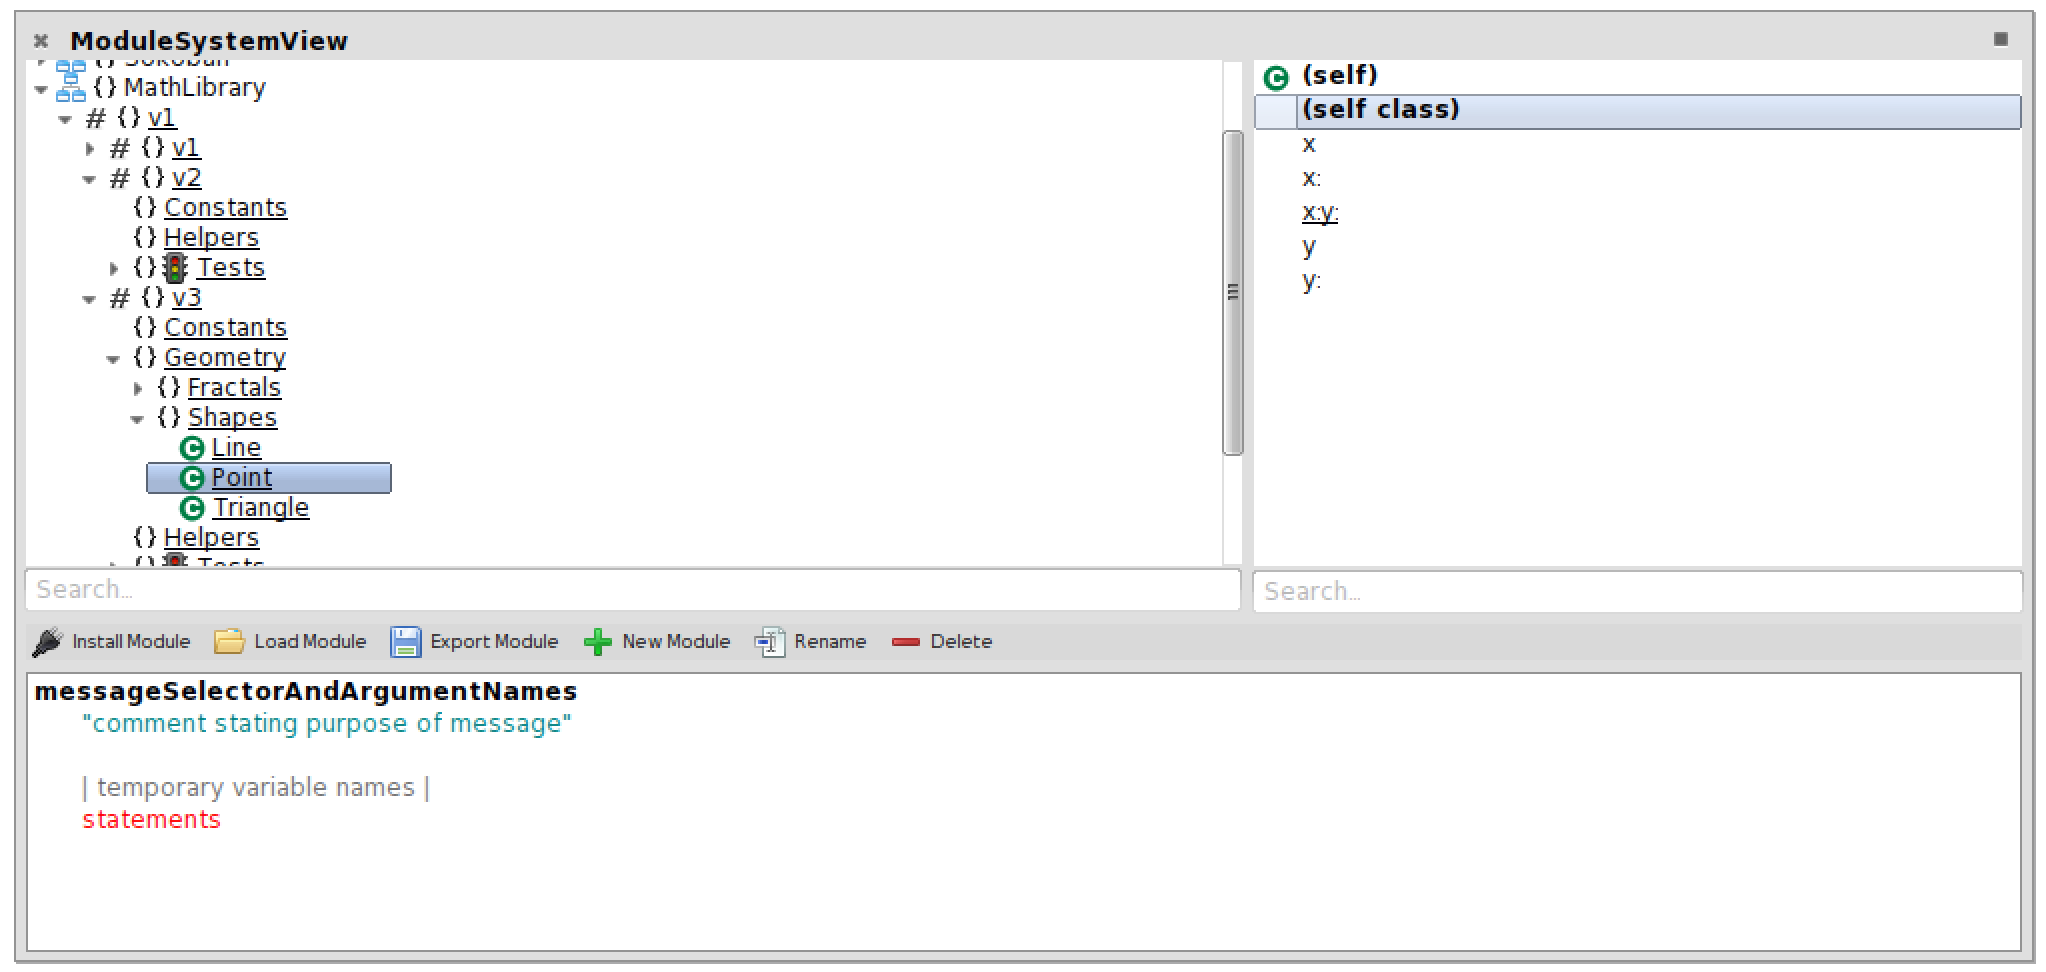
\includegraphics[width=0.8\textwidth]{screenshot_mathlib.png}
\end{table}

\end{explainframe}

\begin{explainframe}{\texttt{ActiveRecordExample}}
  \begin{itemize}
    \item \texttt{Accessors}, \texttt{Printing}, \texttt{Validation} are reusable modules.
    \item Mixin includes are flattened to single inheritance.
  \end{itemize}

\begin{table}
  \centering
  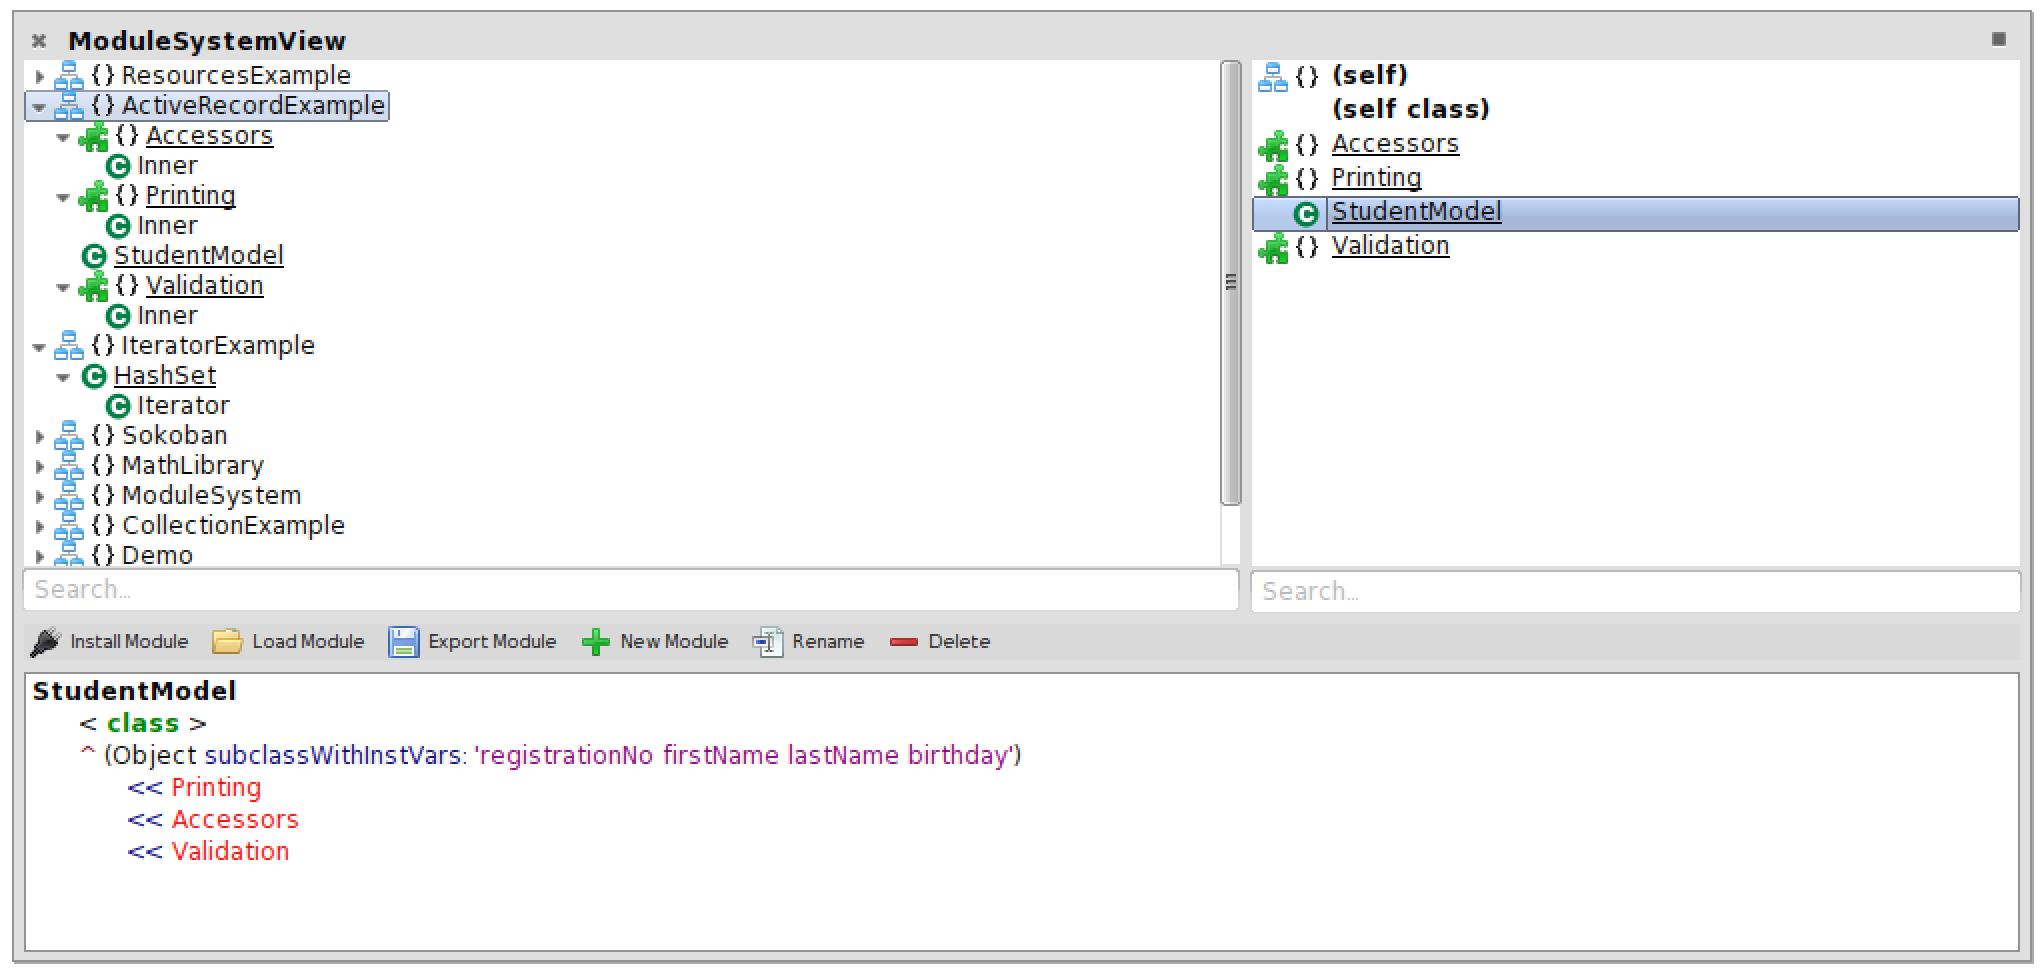
\includegraphics[width=0.8\textwidth]{screenshot_activerecord.png}
\end{table}
\end{explainframe}

\begin{explainframe}{\texttt{CollectionExample}}
  \begin{itemize}
    \item Everything with a \texttt{do:} method can have the collection API.
    \item \texttt{ScuGameTile} is a subclass of \texttt{Morph} and has the \texttt{CollectionMixin} included (alternative: multiple inheritance).
  \end{itemize}

\begin{table}
  \centering
  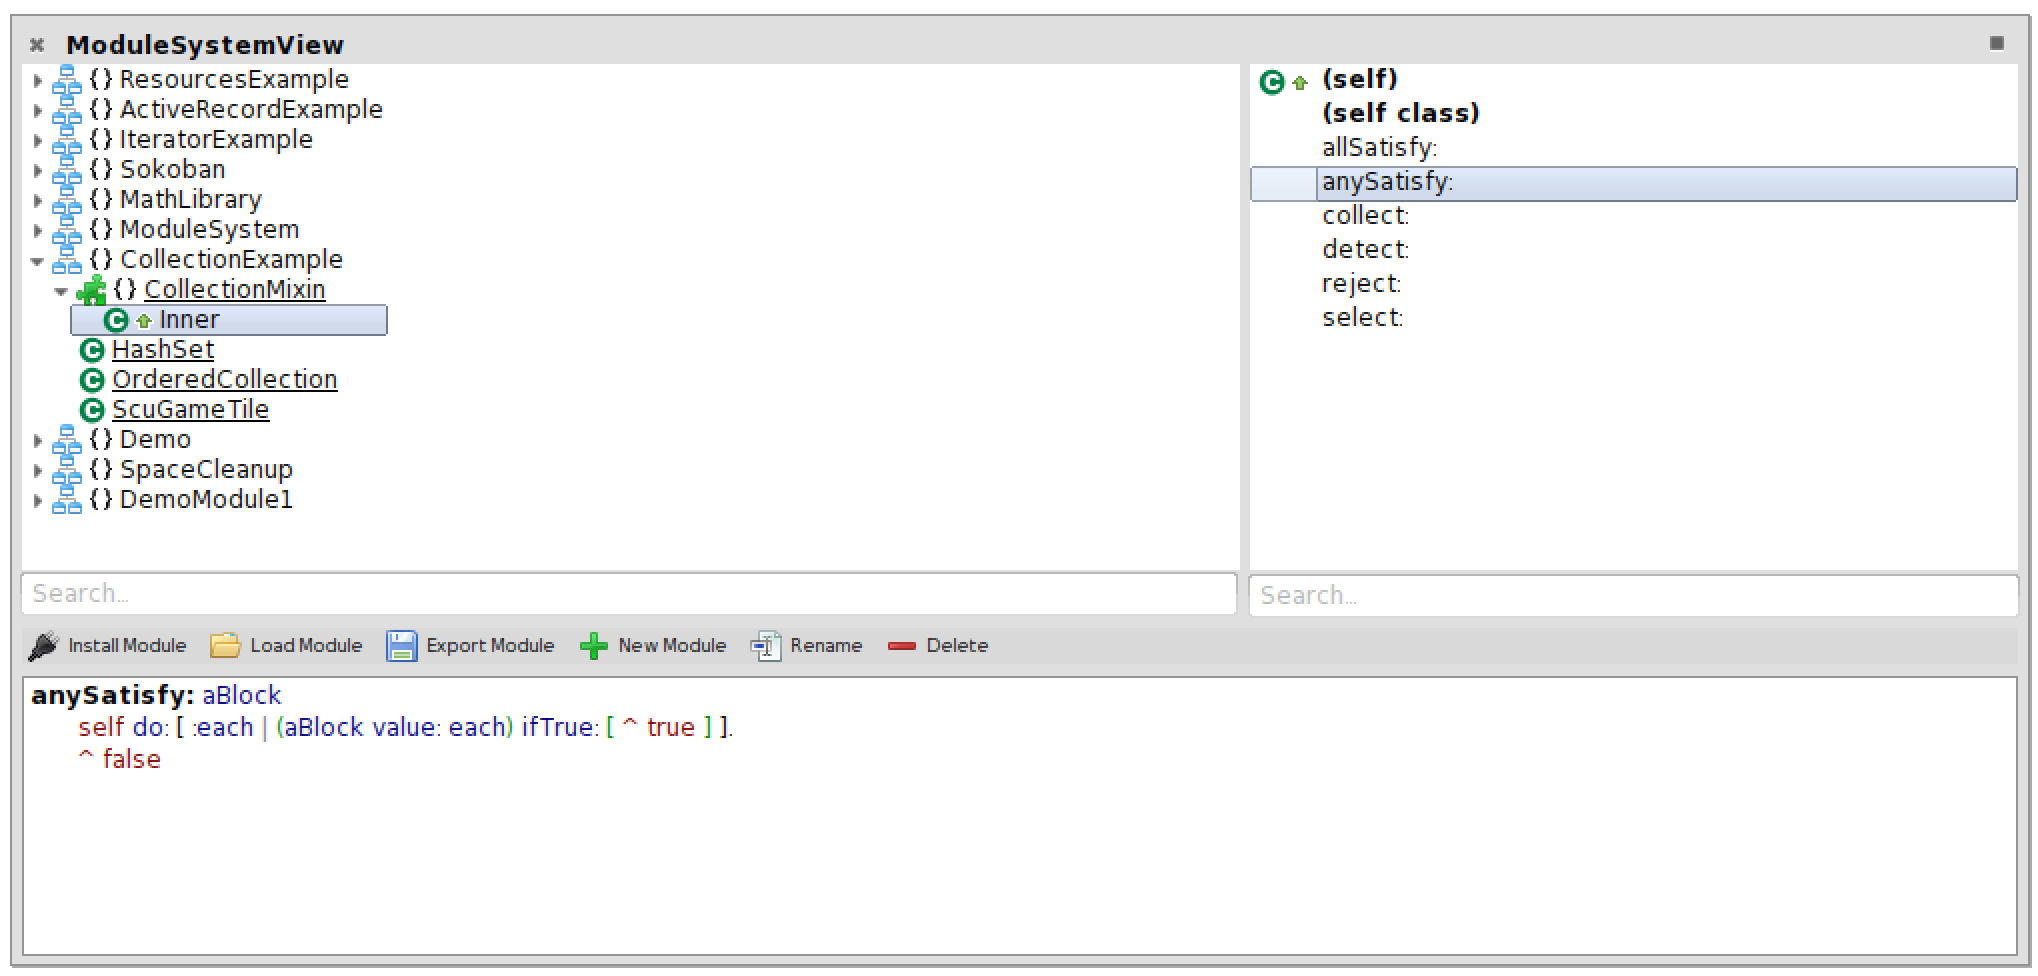
\includegraphics[width=0.8\textwidth]{screenshot_collection.png}
\end{table}
\end{explainframe}

\begin{explainframe}{\texttt{IteratorExample}}
  \begin{itemize}
    \item \texttt{Iterator} is an adapter.
    \item \texttt{Iterator} is an inst-side nested class and bound (belongs to) and instance of \texttt{HashSet}.
    \item Can be used as a form of interface encapsulation: developer can pass an instance of \texttt{Iterator} around instead of \texttt{HashSet}, making sure that nobody accesses private API (unless \texttt{Iterator>>outer} is called).
  \end{itemize}

\begin{table}
  \centering
  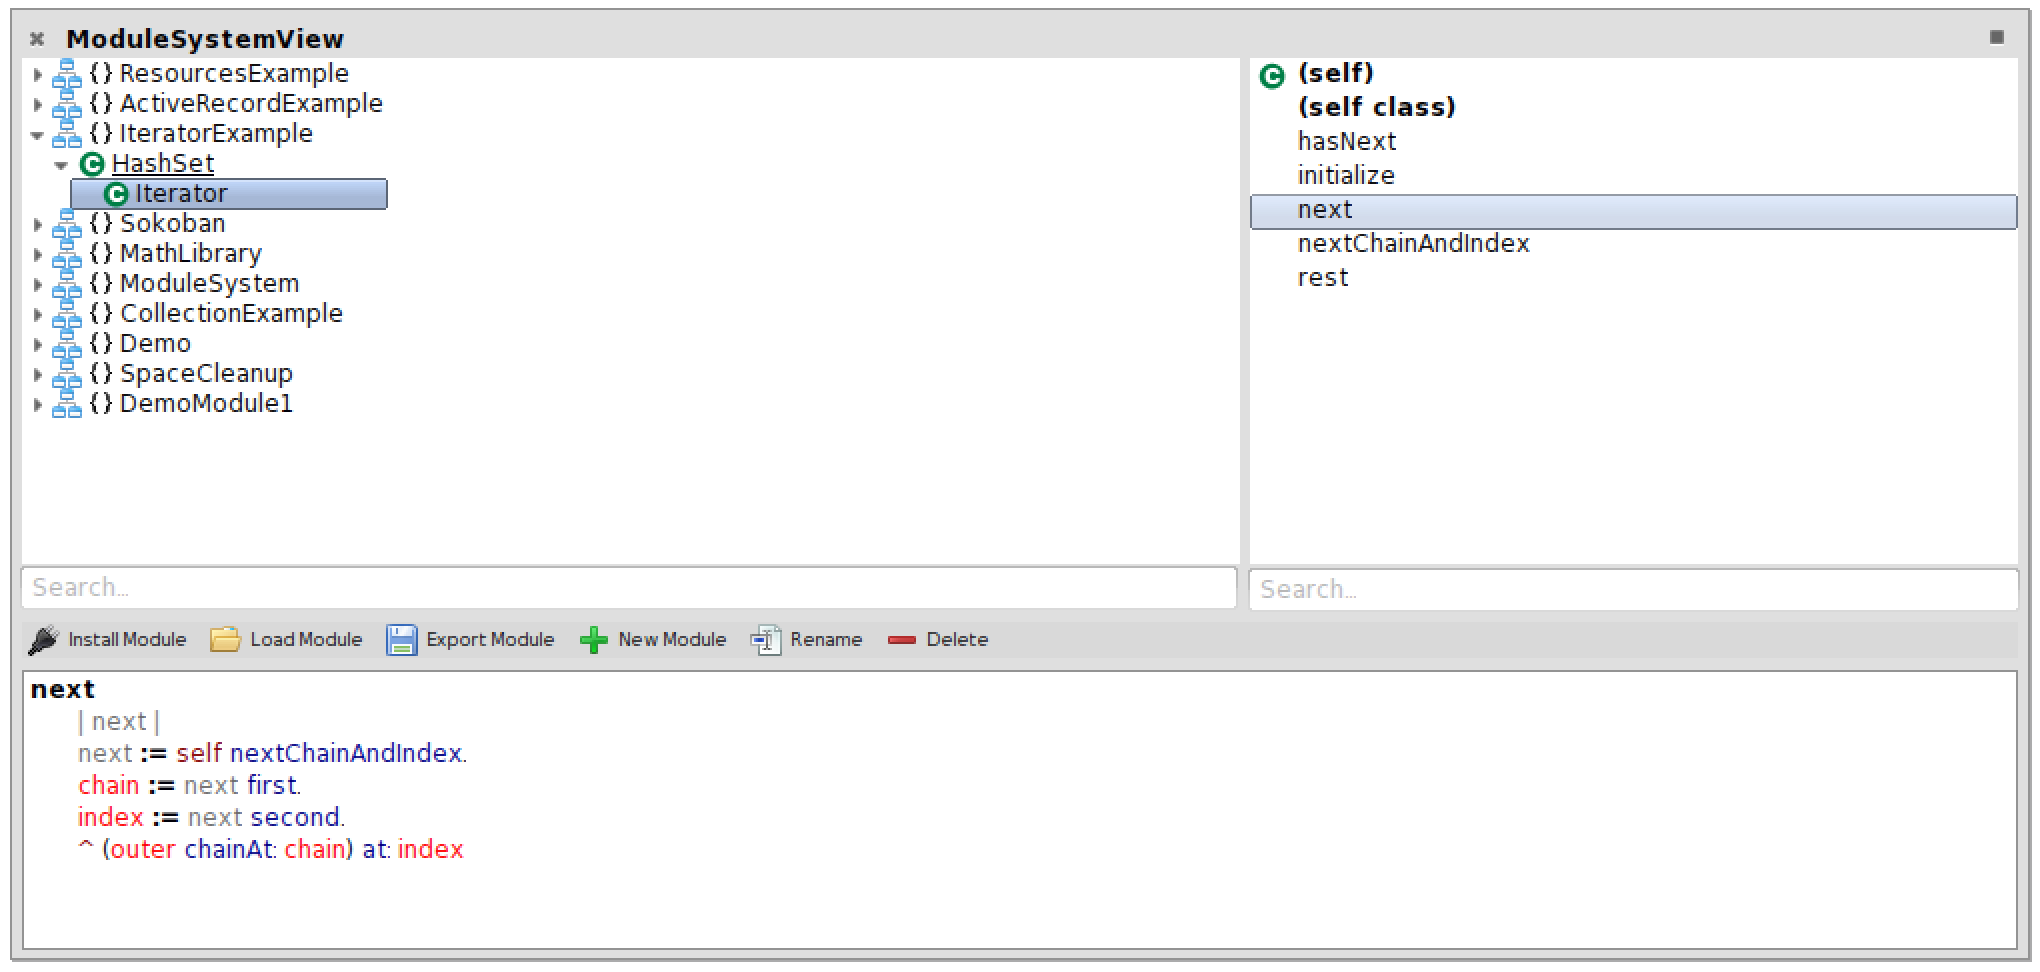
\includegraphics[width=0.8\textwidth]{screenshot_iterator.png}
\end{table}
\end{explainframe}

\begin{explainframe}{\texttt{Sokoban} Resource Management}
  \begin{itemize}
    \item Resources are class members, but not stored as source code.
    \item Resources are exported/imported using \texttt{writeResourceTo:}/\texttt{newFromStream:}.
  \end{itemize}

\begin{table}
  \centering
  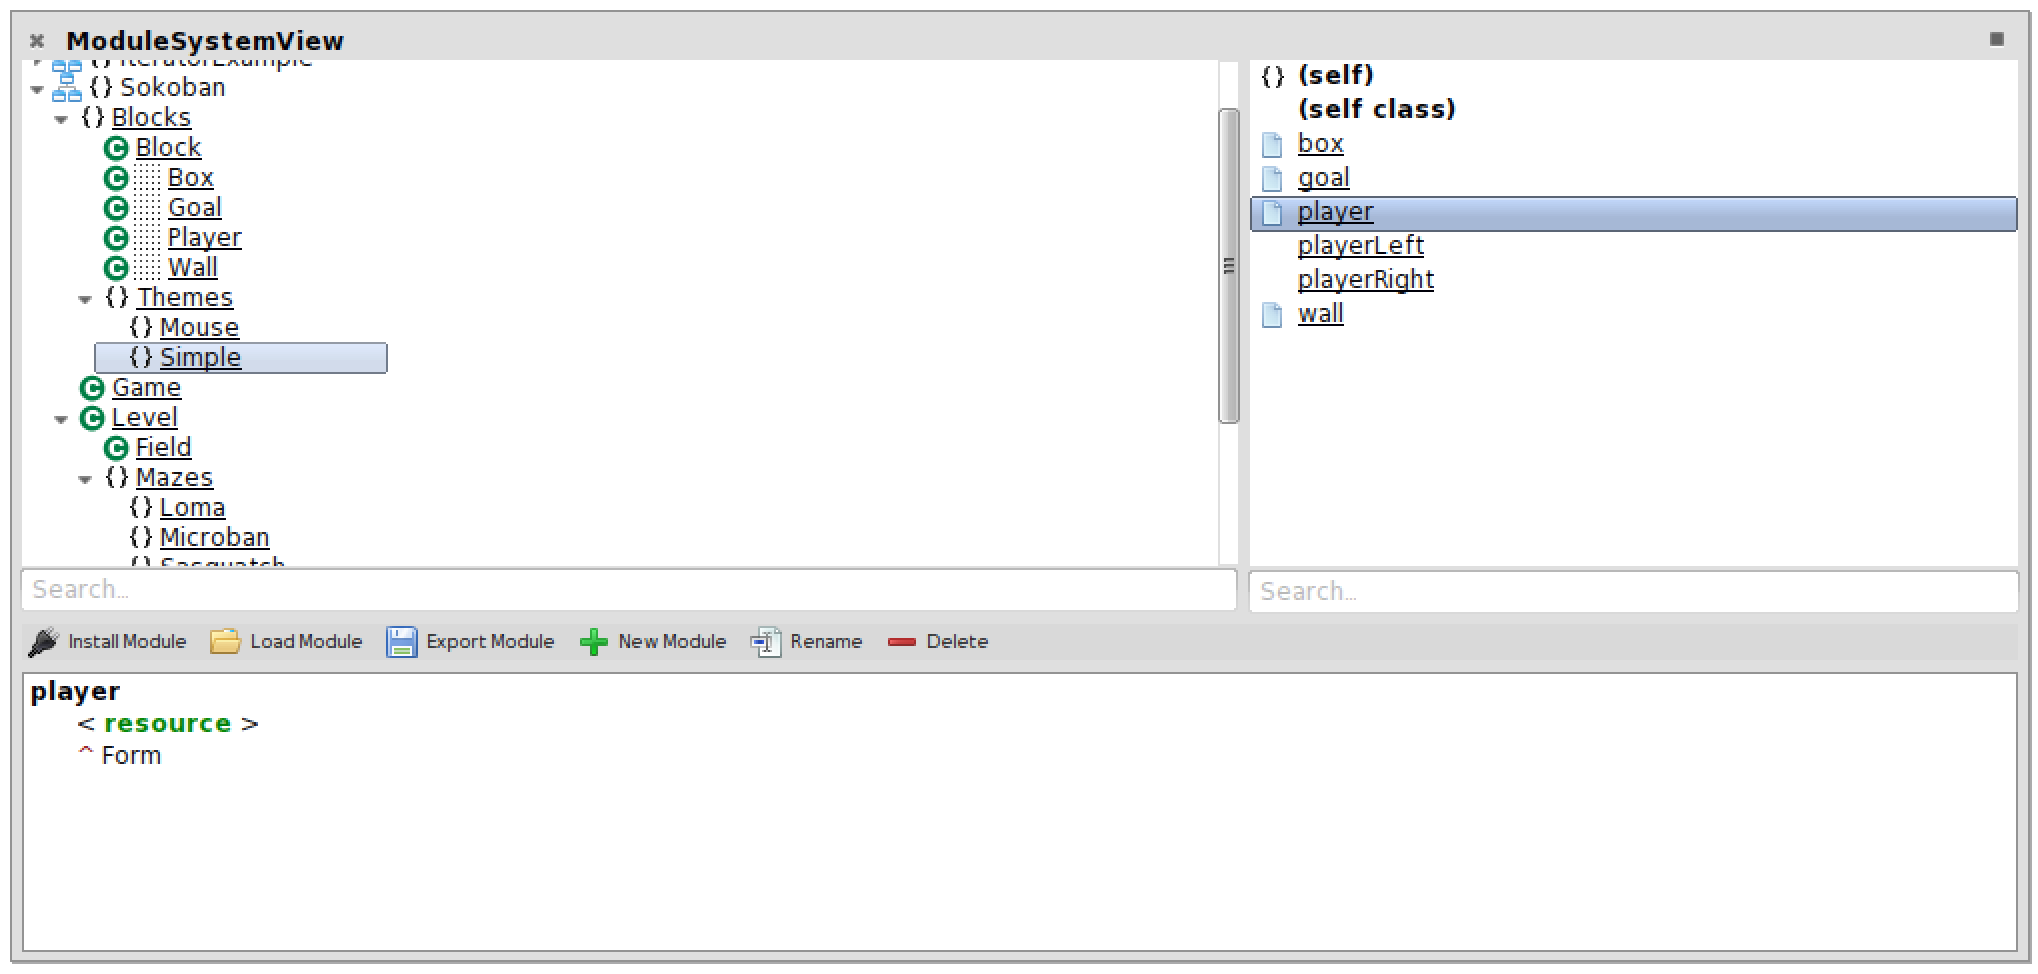
\includegraphics[width=0.8\textwidth]{screenshot_sokoban_res.png}
\end{table}
\end{explainframe}

\begin{explainframe}{\texttt{Sokoban} Fileout/Export}
\begin{minipage}{.35\textwidth}
  \centering
  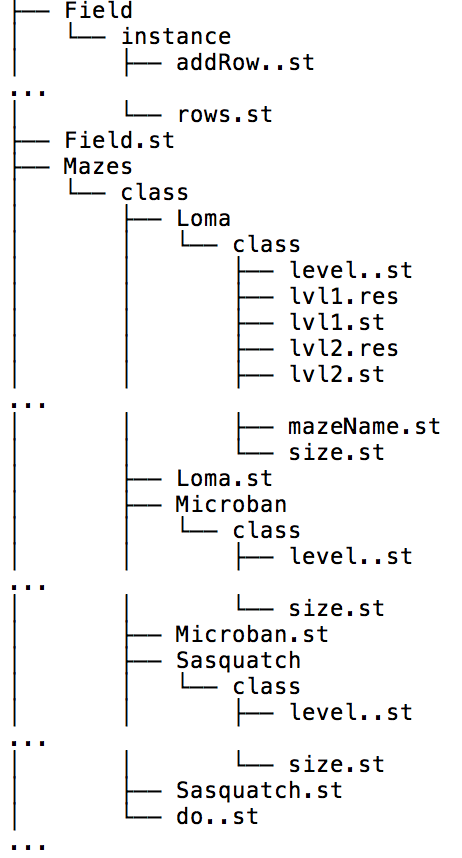
\includegraphics[height=0.85\textheight]{screenshot_sokoban_export.png}
\end{minipage}% This must go next to `\end{minipage}`
\begin{minipage}{.05\textwidth}
\qquad
\end{minipage}% This must go next to `\end{minipage}`
\begin{minipage}{.6\textwidth}
\begin{itemize}
  \item Class = new directory + corresponding method file.
  \item Method = source code file.
  \item Resource = resource file + corresponding method file.
  \item \texttt{classname/class} for class-side, \texttt{classname/instance} for inst-side.
  \item System provides \emph{load} and \emph{save} functionality, but no merge (should be done via underlying version control system).
\end{itemize}
\end{minipage}
\end{explainframe}

\section{Implementation}

\begin{frame}{Lazy Class Generation}
\centering
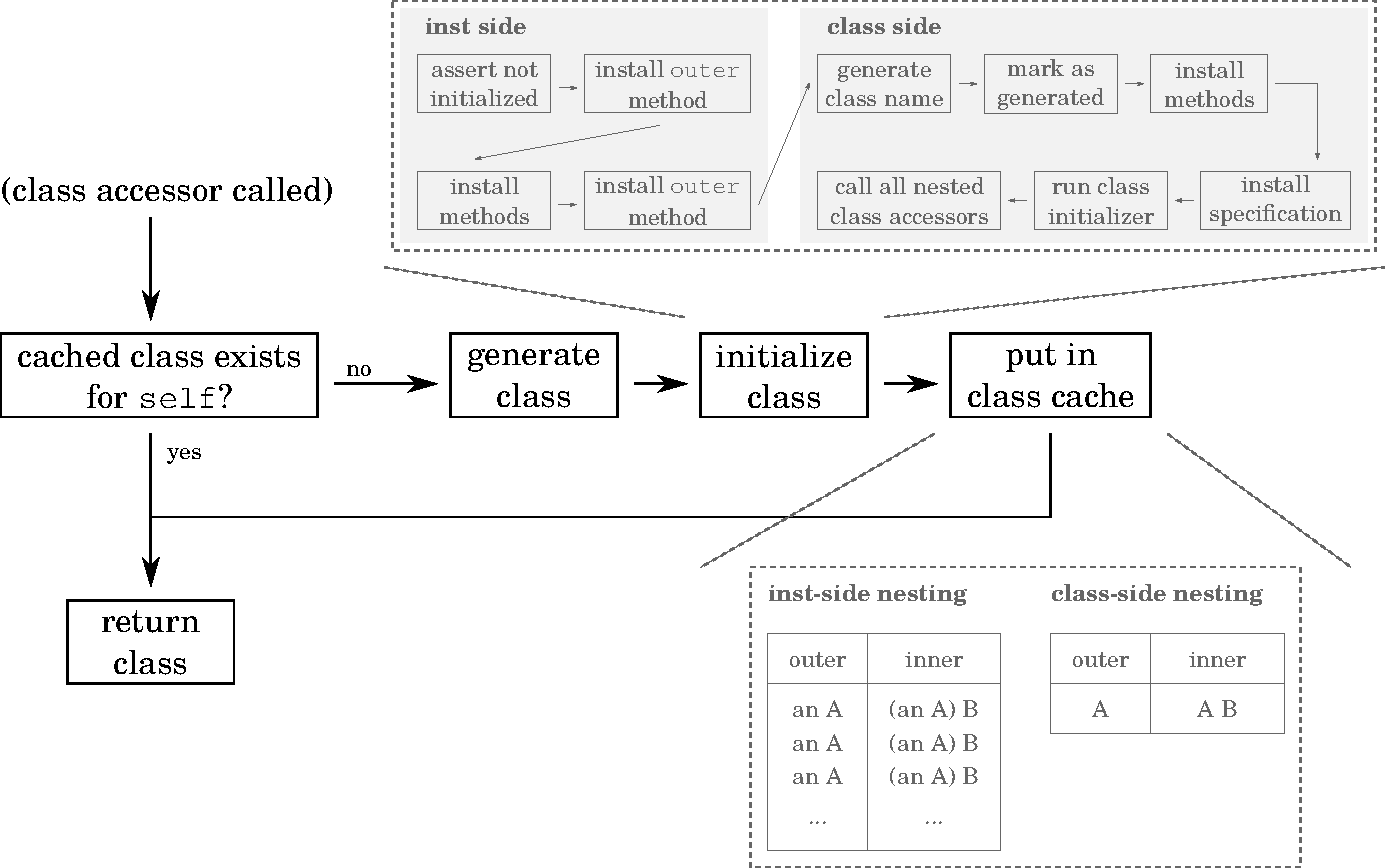
\includegraphics[width=\textwidth]{lazy_class_gen.pdf}
\end{frame}

\begin{explainframe}{Lazy Class Generation}
\begin{itemize}
  \item Class accessor generates and caches nested class.
  \item Cache is a \texttt{WeakIdentityKeyDictionary} (instance variable of corresponding \texttt{MethodSpecification}).
  \item All \emph{entirely} class-side nested classes are initialized upon module instantiation (except for class-side nested classes that have an inst-side ancestor).
\end{itemize}
\end{explainframe}

\begin{frame}{Meta-Model and Instantiation}
  \centering
  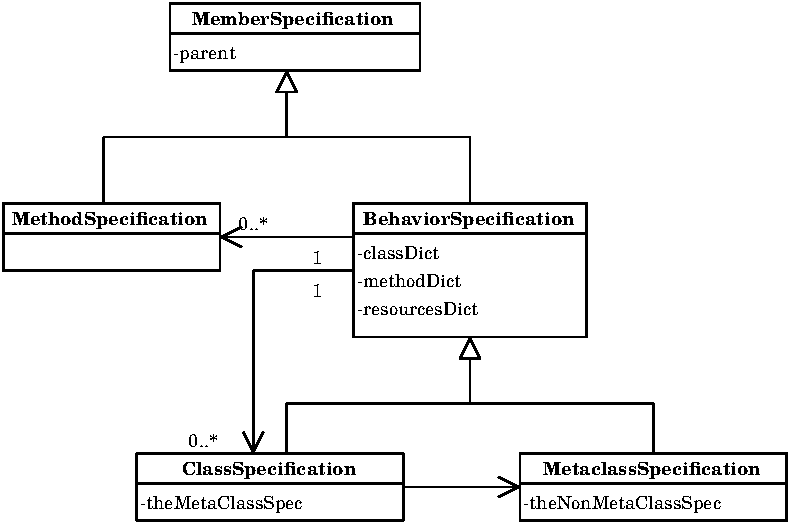
\includegraphics[width=0.8\textwidth]{metamodel.pdf}
\end{frame}

\begin{frame}{Early vs. Late \texttt{outer} Binding}
\begin{table}
\centering
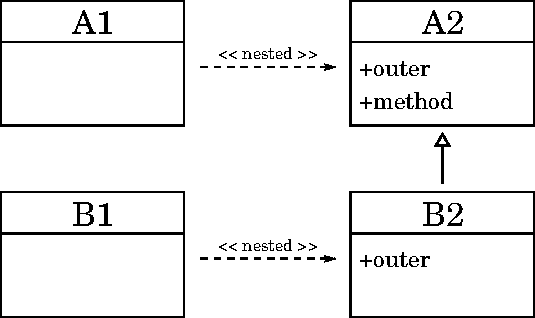
\includegraphics[width=0.7\textwidth]{outer_binding.pdf}
\end{table}

\begin{itemize}
  \item Method \texttt{outer} is late bound.
  \item Keyword \texttt{outer} is early bound.
\end{itemize}
\end{frame}

\begin{explainframe}{Early vs. Late \texttt{outer} Binding}
\begin{lstlisting}
A2>>method
  ^ { outer. self outer}

A2 new outer.
" returns { A1. A1. } "

B2 new outer.
" returns { A1. B1. } "
\end{lstlisting}

\begin{itemize}
  \item \texttt{outer} keyword is bound as \texttt{CompiledMethod} literal.
  \item Early binding is useful for class binding, to avoid accidential name capturing.
\end{itemize}
\end{explainframe}

\begin{frame}{Class Lookup}
  \begin{table}
    \centering
    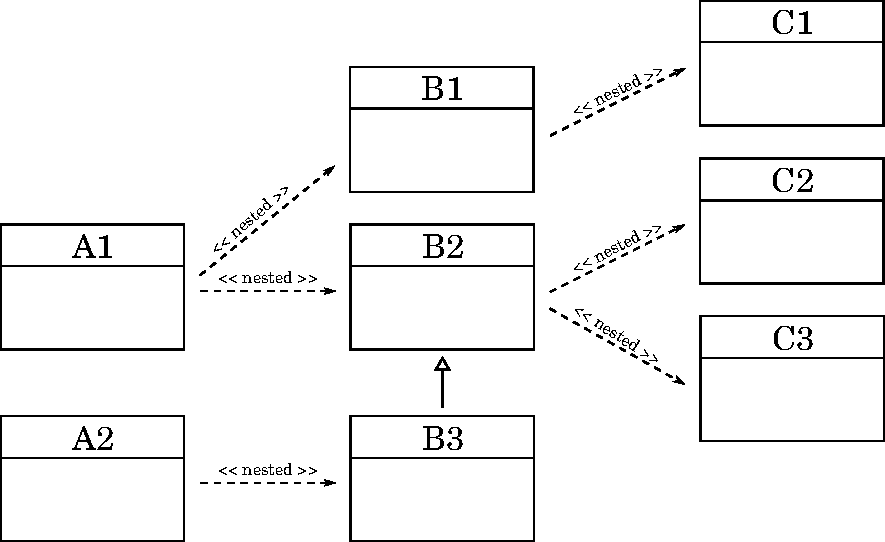
\includegraphics[width=0.75\textwidth]{class_lookup.pdf}
  \end{table}

  \begin{itemize}
    \item Order: \texttt{self}, \texttt{outer}, \texttt{outer outer}, \ldots
    \item References to classes contained in ancestors are early bound (unless \texttt{self} send).
    \item References to nested classes of myself are late bound.
  \end{itemize}
\end{frame}

\begin{explainframe}{Class Lookup}
\begin{lstlisting}
B2>>method
  ^ { A1.   " early bound "
      B1.   " early bound "
      B2.   " early bound "
      C1.   " lookup fails "
      C2.   " late bound "
      C3.   " late bound "
    }
\end{lstlisting}

\begin{itemize}
  \item Early bound ancestors lookup is identical to using \texttt{outer} keyword: \\ \texttt{B2 == outer B1} in \texttt{B2}.
  \item Late bound lookup can be forced using self sends: \texttt{self outer B1} (have to specify full path).
\end{itemize}
\end{explainframe}

\begin{frame}[fragile]{Class Generators (Mixins)}
\begin{figure}
  \centering
  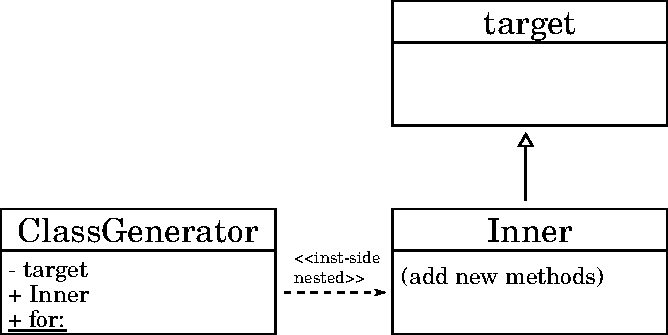
\includegraphics[width=0.5\textwidth]{class_generator.pdf}
\end{figure}

\begin{lstlisting}
ModelBase << Validation << Persistance
\end{lstlisting}
\end{frame}

\begin{explainframe}{Class Generators (Mixin)}
\begin{lstlisting}
CollectionMixin := Object subclassWithInstVars: 'target'.

CollectionMixin>>Inner>>collect: aBlock
  ^ ...

Class>> << mixin
  ^ (mixin new
    target: self;
    Inner) subclass
\end{lstlisting}
\end{explainframe}

\begin{frame}{Versioning Helpers}
  \begin{itemize}
    \item Use class-side nested classes as version containers.
    \item \texttt{MathLibrary v1 v2}.
    \item Development process: write code in \texttt{MathLibrary dev}, system provides a way to copy \texttt{dev} and add it as a new version.
  \end{itemize}
\end{frame}

\begin{frame}{Module System Base Library}
  Subclass from these classes to build \ldots
  \begin{itemize}
    \item \texttt{ClassGenerator}: \ldots mixin modules, providing helper methods.
    \item \texttt{Module}: \ldots top-level classes.
    \item \texttt{Namespace}: \ldots non-instantiable classes (pure namespace classes).
    \item \texttt{ResourceDictionary}: (a mixin module to use a class like a dictionary).
    \item \texttt{TestCaseHolder}: \ldots test cases (container for \texttt{TestCase} subclasses).
    \item \texttt{Tests}: (contains tests for the module system iteself).
    \item \texttt{Uninstantiable}: (a mixin module marking a class as uninstantiable (namespace)).
    \item \texttt{Version}: \ldots versions/releases.
    \item \texttt{Versioning:} (a mixin module providing convenience methods (e.g. \texttt{latest})).
    \item \texttt{VersioningModule}: \ldots top-level classes containing versions.
    \item \texttt{VersioningVersion}: \ldots versions containing versions.
  \end{itemize}
\end{frame}

\begin{clearexplainframe}
  \centering
  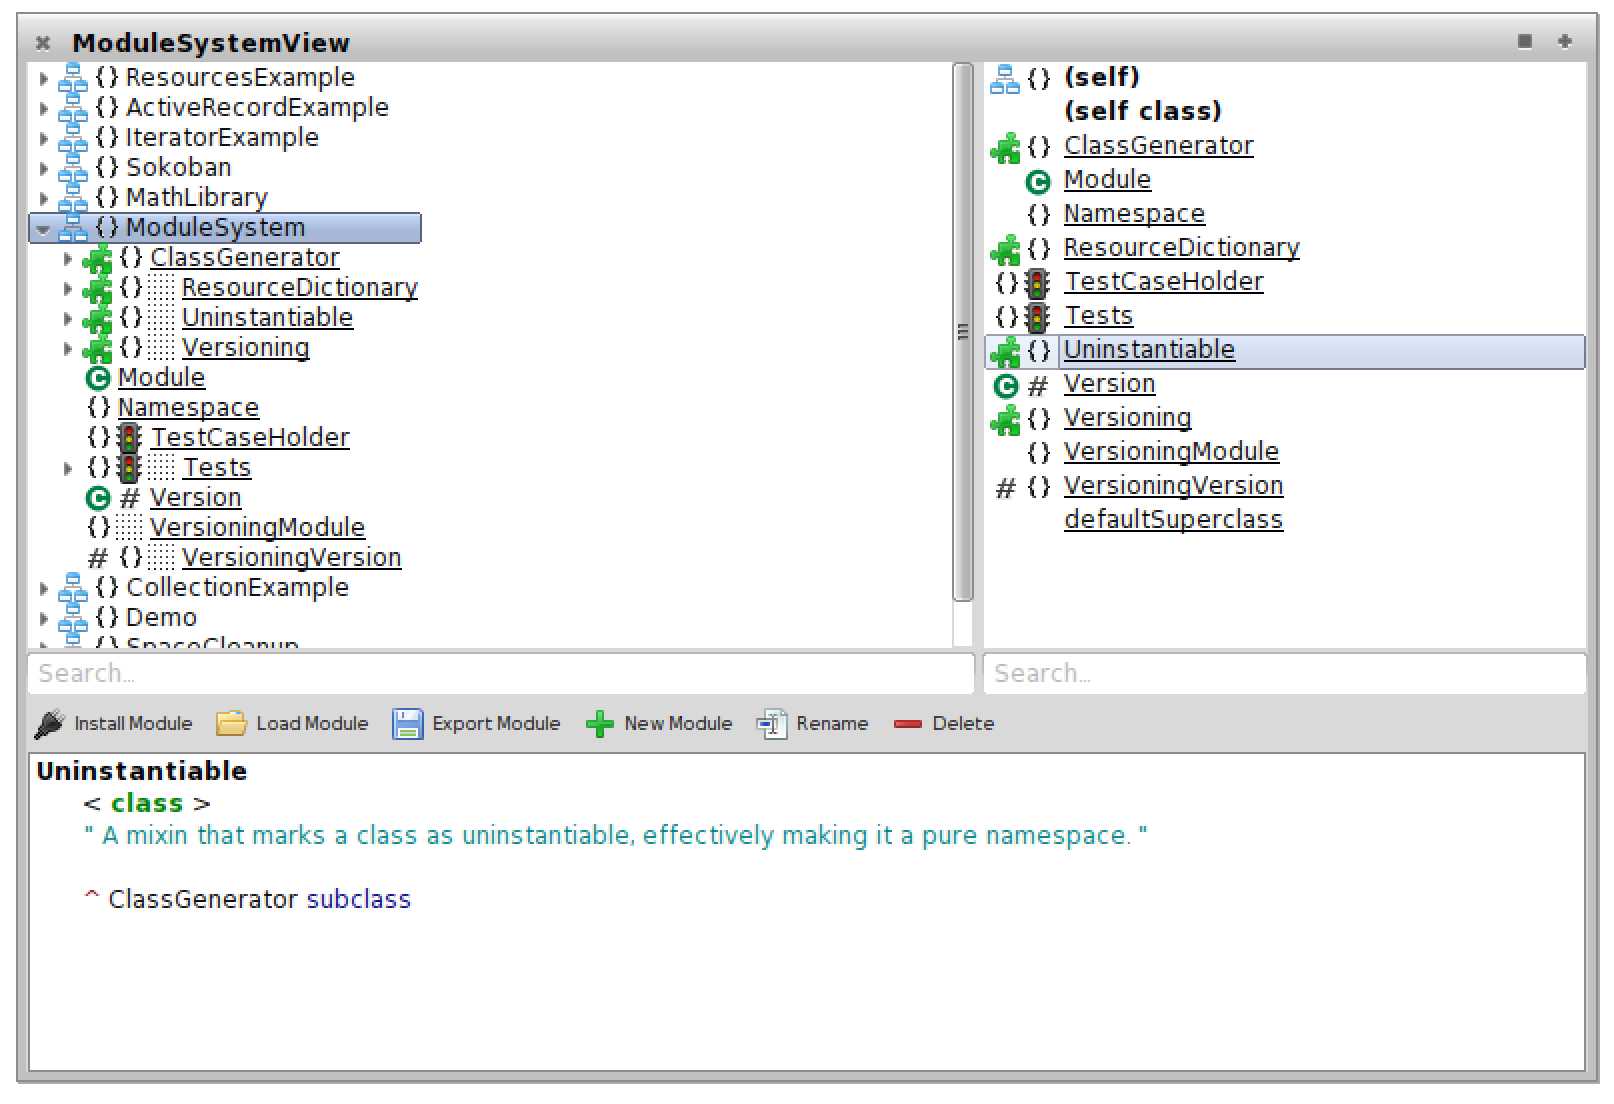
\includegraphics[width=\textwidth]{screenshot_ms.png}
\end{clearexplainframe}


\begin{explainframe}{Module System Base Library}
\begin{lstlisting}
Namespace := Object subclass << Uninstantiable.
TestCaseHolder := Object subclass << Uninstantiable.
Tests := TestCaseHolder subclass.
VersioningModule := Module subclass << Versioning.
VersioningVersion := Version subclass << Versioning.
\end{lstlisting}
\end{explainframe}

\section{Integration in Squeak}
\begin{frame}{Integration in Squeak}
  \centering
  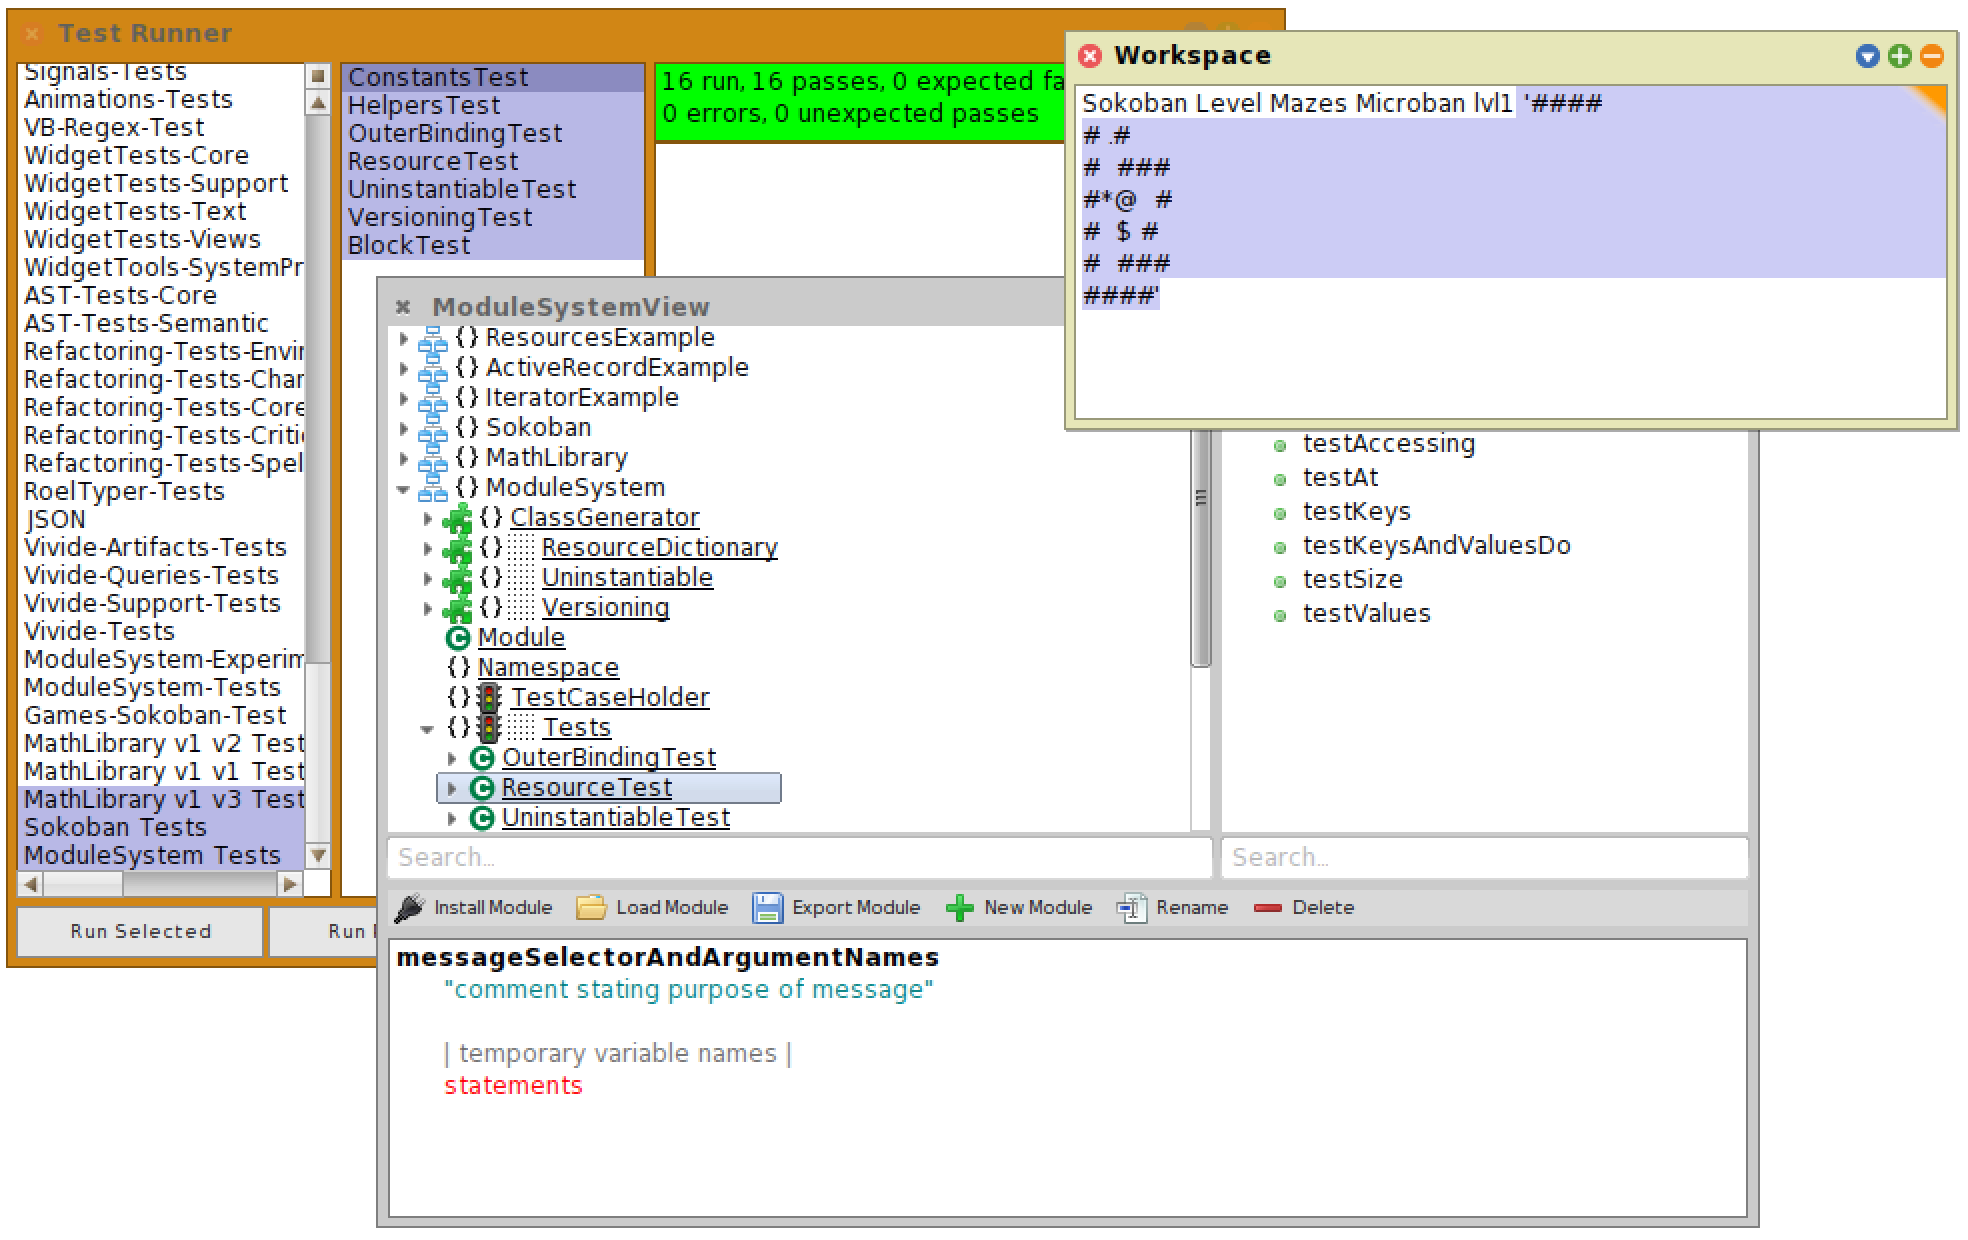
\includegraphics[width=\textwidth]{screenshot_integration.png}
\end{frame}

\begin{frame}{Integration in Squeak}
\begin{itemize}
  \item Compatible to Squeak-Trunk.
  \item New Vivide-based system browser (old browser is incompatible).
  \item Custom import/export format wit Git support (Monticello is incompatible).
  \item Testrunner can be used as normal.
  \item Debugger works, but shows transformed source code.
\end{itemize}
\end{frame}

\section{Next Steps}
\begin{frame}{Next Steps}
  \begin{itemize}
    \item Class migration and live system editing.
    \item COP layer for extension methods.
    \item Solve performance issues during model instantiation.
    \item UI polishing and tool adaptation (debugger, sender/implementors/... etc.).
  \end{itemize}
\end{frame}

\end{document}
